\section{Architecture du programme}

\par
Dans cette section nous aborderons l'architecture du programme. C'est-à-dire la façon dont est organisé notre code et notamment les choix d’implémentation que nous avons effectués. Pour rappel, notre objectif est de générer un arbre rythmique et de récupérer la liste des accords et symboles musicaux pour réaliser l'affichage de la partition musicale.

\subsection{Analyse du problème}

\par
Le format \emph{MusicXML}, et plus généralement une partition musicale, peut comporter énormément de symboles différents. C'est pour cela que nous avons du nous adapter à la structure très "personnalisable" et penser le code pour qu'il soit très malléable. Pour ce faire, nous avons gardé un niveau d'abstraction assez élevé pour pouvoir implémenter chaque symbole en modifiant le minimum de code. Lors de la réflexion qui a découlé de ce constat, nous avons pu observer deux types de symbole : les symboles unaires et les symboles binaires.
\par
Les symboles unaires sont assez simple à implémenter dans le sens où il n'influence, pour la plupart du temps, qu'une seule note. Il nous suffit donc de les stocker dans ladite note.
\par
En ce qui concerne les symboles binaires, l'implémentation est beaucoup plus contraignante. Certains symboles, comme les groupes de croches, ont des marqueurs de début, de continuation et de fin, alors que d'autres, comme les groupes de liaison, n'ont qu'un début et une fin. Cela nous oblige donc à faire du sur-mesure pour certains symboles.
\par
Il demeure cependant des symboles qui peuvent concerner une mesure comme la partition. La balise \emph{<metronome>} par exemple est renseignée dans la mesure de la même façon qu'une note. Il faut donc prendre en compte ces exceptions.


\subsection{Architecture générale}

\par
Le programme se divise en trois parties. La première étant le parser. Cette partie permet au programme de disposer d'un \emph{DOM} à partir d'un fichier MusicXML. La seconde partie est la représentation objet des données contenues dans le \emph{DOM}. Et enfin la troisième partie est l'arbre rythmique qui pourra être généré à partir de la représentation objet de la partition.

\subsection{Parsing du fichier MusicXML}

\par
La première étape est de parser le document afin d'extraire les informations qu'il contient. C'est là qu'interviennent les éléments contenus dans le package \emph{pstl.musicxml.parsing}. Nous avons décidé d'encapsuler le parser XML natif de Java dans une classe \emph{XMLParser}. Ce choix est motivé pour plusieurs raisons.

\par
Tout d'abord, pour ne laisser apparent que les fonctions du parser de Java que nous allons réellement utiliser afin de limiter le risque que nous, ou un utilisateur tiers, fasse usage du parser d'une mauvaise façon. Nous avons aussi fait ce choix pour simplifier l'utilisation de la classe pour que la création du parser qu'elle encapsule se fasse de la même façon à chaque fois. Et enfin ce choix a été rendu nécessaire à cause de \emph{Relax NG}. En effet comme nous ne faisons appel ni aux fichiers \emph{DTD} ni aux fichiers \emph{XML Schema}, il nous faut effectuer un prétraitement pour éliminer les références aux \emph{DTD} du fichier à parser. Vous pourriez vous demander pourquoi ne pas simplement utiliser les \emph{DTD} pour valider le document ? La raison est simple, la plupart des fichiers font référence aux \emph{DTD} en ligne fournis par MusicXML. Or ces derniers n'autorisent que les navigateurs web à accéder à de tels fichiers. Les possibilités qui s'offraient à nous étaient les suivantes : se faire passer pour un navigateur en modifiant quelques variables d’environnement. Cela aurait eu pour désavantage tout d'abord de ne pas être très rapide, l'accès à aux \emph{DTD} par réseau n'est pas très rapide comparé à un accès local. Nous jugions d'autre part la méthode peu honnête. En effet si l'organisation derrière MusicXML ne permet pas cela pour des raisons que nous imaginons financières (par cela j'entends le coût engendré par la maintenance des serveurs), il n'aurait pas été juste d'outrepasser leurs instructions. Et enfin le dernier choix non retenu était celui de faire appel à des \emph{DTD} stockées localement. Cette méthode a été écartée bien que conseillée dans la documentation du format MusicXML car elle impliquait des redirections d'URI ce qui aurait fortement complexifié la création du parser.

\par
C'est donc pour toutes ces raisons que nous avons choisi d'utiliser \emph{Relax NG}. De plus, les fichiers décrivant la grammaire de MusicXML sont disponibles en ligne et l'auteur, qui les a déposés sur un projet GitHub \cite{relaxng_for_musicxml}, a fait preuve d'une certaine exhaustivité lors de la rédaction de ces derniers.

\par
Ce parser nous permet de disposer d'un \emph{DOM} (qui a pour nom de classe \emph{Document} avec Java) qui pourra être parcouru plus tard. Le schéma suivant récapitule les étapes pour passer du document XML au DOM.


\begin{figure}[!h]
\centering
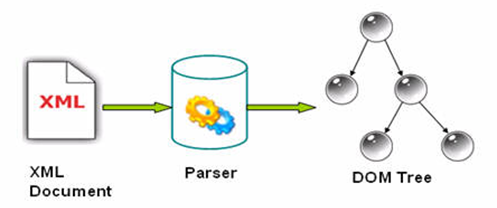
\includegraphics[width=0.5\textwidth]{parsing_xml_to_dom.png}\\[1cm]
%source : http://www.amfastech.com/2014/11/complete-tutorial-on-selecting-best-xml-parser.html
\caption{Parsing d'un document XML en DOM}
\end{figure}


\subsection{Représentation objet de la partition}

\par
Nous aurions pu nous satisfaire du \emph{Document} retourné par le parser pour générer notre arbre rythmique mais cela aurait posé plusieurs problèmes. Tout d'abord la manipulation du \emph{DOM} n'est pas aisée. Cette structure de données basé sur des nœuds qui contiennent des fils, attributs et leur contenu textuel, doit être exploré d'une façon assez lourde à cause en partie du fait qu'un nœud n'est pas nativement un objet itérable comme les \emph{Collections} de Java par exemple. D'autre part, toutes les données contenues dans ces nœuds sont considérées comme des chaînes de caractère qui nécessitent un parsing et donc une manipulation assez verbeuse. De ce fait, il est plus simple pour nous de parcourir ce \emph{Document} une seule fois et d'extraire les données qu'il contient dans une structure de données plus aisément manipulable dans Java. Cela permet par exemple d'éviter des erreurs lors du développement des autres fonctionnalités de l'application qui se basent sur ces informations. Nous utilisons donc un ensemble de méthodes contenus dans la classe \emph{ScoreUtils} pour convertir notre \emph{Document} en instance de \emph{Score}.

\begin{figure}[!h]
\centering
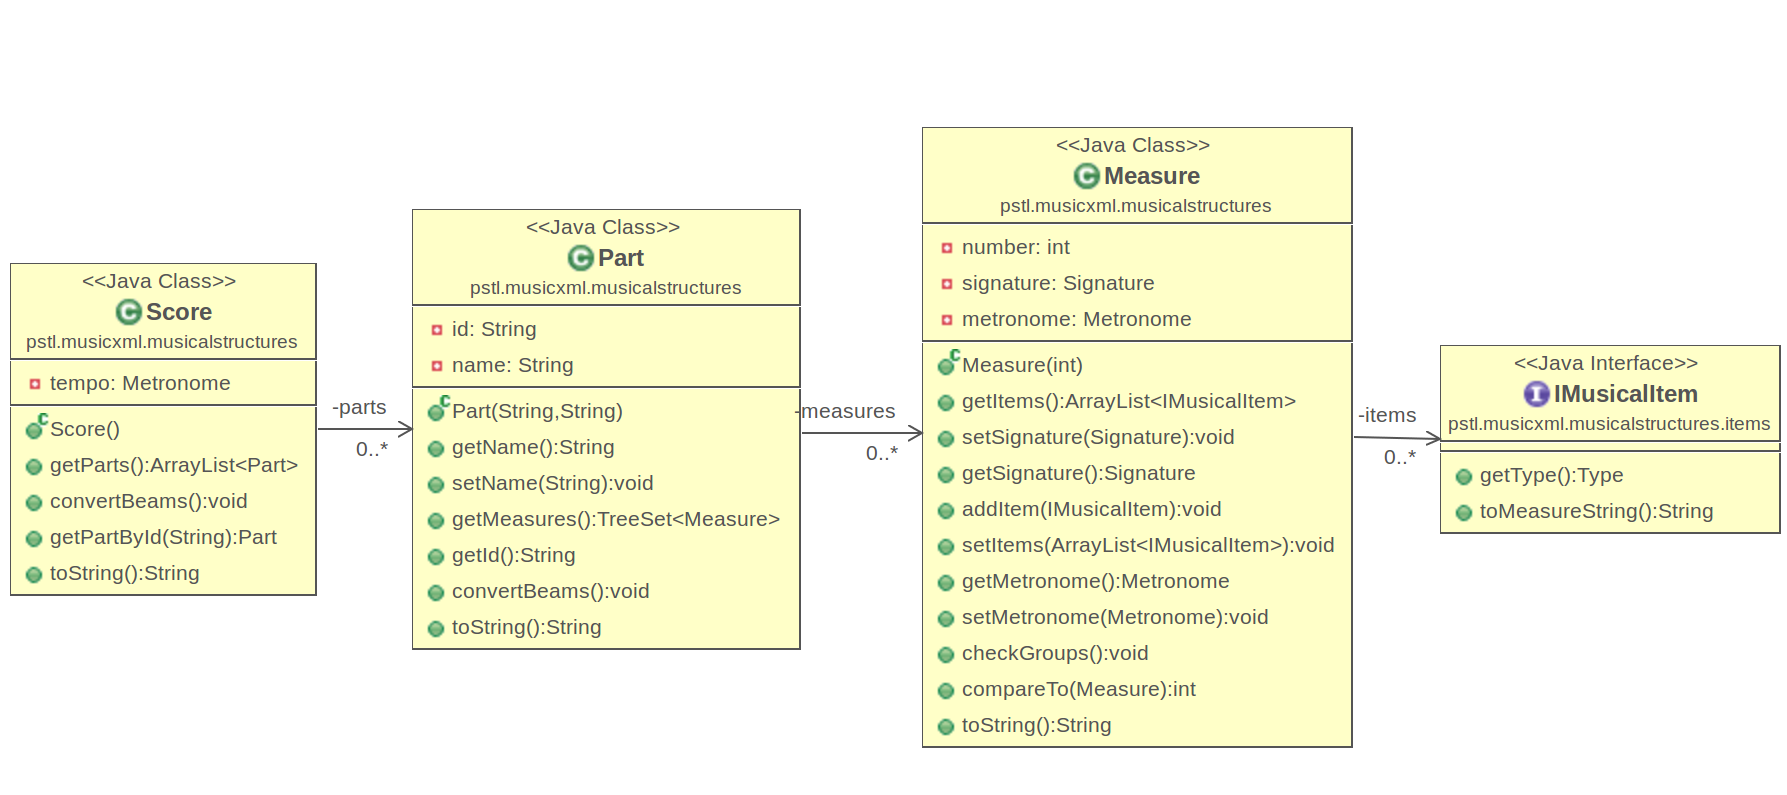
\includegraphics[width=1\textwidth]{muscicalStructureClassDiag.png}\\[1cm]
%source : Alexandre
\caption{Structure d'une partition sous forme d'un diagramme de classe UML}
\end{figure}

\par
\emph{ScoreUtils} intègre aussi une partie très importante : la récupération des symboles contenus dans la partition. En effet, une partition n'est pas seulement un ensemble de notes, il contient aussi un grand nombre de symboles ayant tous des significations très différentes pouvant aussi bien influencer la tonalité de la note que sa durée.

%Mettre des figures pour expliciter les partitions ? Un diagramme de class par exemple ?
%TODO établir un vrai package pour les partitions.

\par
La structure de données que nous avons élaborée se compose de la façon suivante : l'élément qui va contenir toutes les informations est la classe \emph{Score}. Une\emph{Score} contient une liste de \emph{Parts} qui l'on peut qualifier de \emph{Voix} en français. Chaque \emph{Part} contient un nom, un identifiant ainsi qu'une liste de \emph{Measures} (mesure) qui contient elle-même un numéro, une \emph{Signature}, une liste de \emph{IMusicalItem} et un \emph{Metronome} correspondant au tempo.

\par
\emph{IMusicalItem} est la super classe de bon nombre d'éléments que nous pouvons qualifier de bout de chaîne comme les \emph{Note}, \emph{Rest} (silence) ou encore les \emph{Tie} (liaison). Mais ce n'est pas tout, les groupes de \emph{IMusicalItem} sont également des \emph{IMusicalItem}. Cela nous permet entre autre de pouvoir imbriquer des groupes de \emph{IMusicalItem}. Dans les premières versions de cette partie du code, il n'y avait pas de liens entre les mesures et les groupes. Nous nous sommes rapidement rendu compte que la mesure et le groupe étaient à peu de chose près la même chose. Nous avons donc décidé qu'il serait mieux que le mesure soit aussi un groupe pour limiter la duplication de code. Un groupe peut représenter des croches liées ou encore un \emph{triolet}.

\par
Pour chaque symbole musical, une classe lui est associée. Le symbole peut être unaire ou binaire. Les symboles unaires sont liés à une seule note, tel que les points d'orgues. Les symboles binaires sont liés à 2 notes, comme les liaisons. Pour chaque note, on récupère tous les symboles qui lui sont associés, on créé les objets intermédiaires et on les ajoute à l'objet \emph{Note}.


\begin{figure}[!h]
\centering
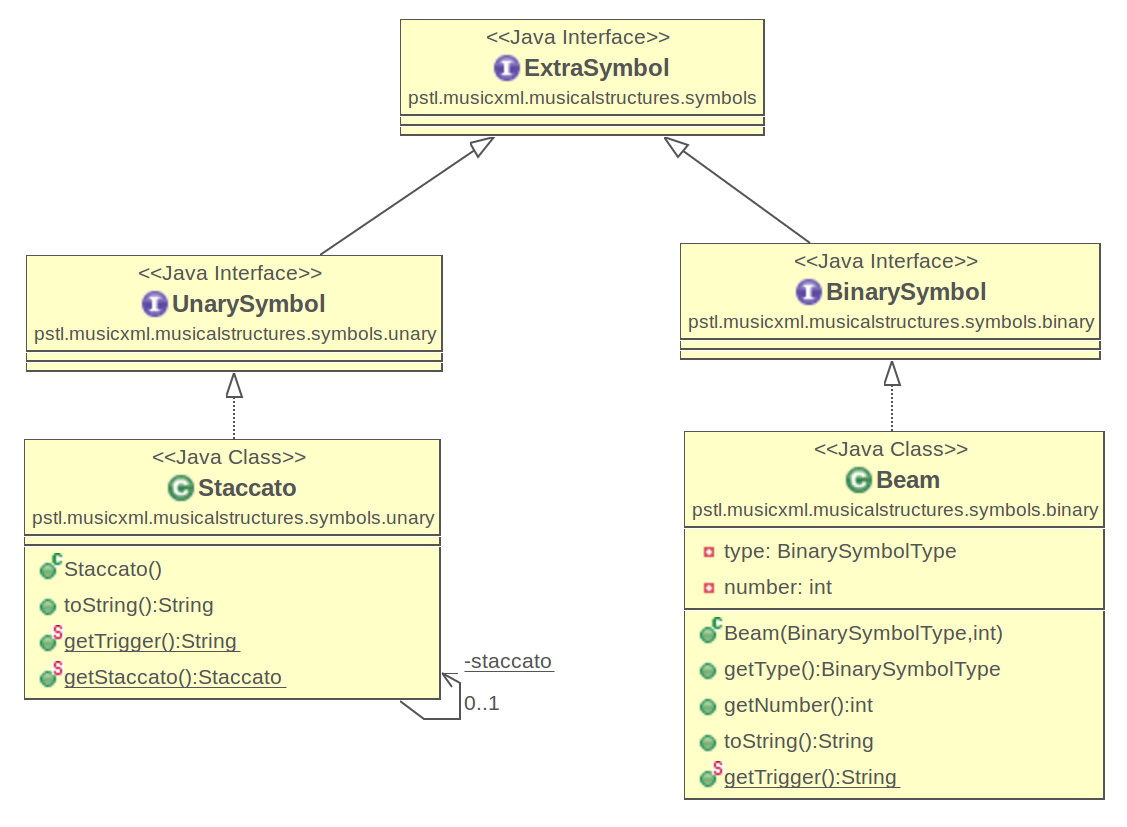
\includegraphics[width=1\textwidth]{symbolsClassDiagram.png}\\[1cm]
%source : Alexandre
\caption{Structure des symboles sous forme d'un diagramme de classe UML}
\end{figure}


\par
La création de l'objet \emph{Score} se fait en deux étapes. Tout d'abord, nous récupérons les données brutes dans le \emph{Document} que nous mettons dans l'objet \emph{Score} final. Une fois toutes ces données à disposition, nous pouvons créer les groupes en fonction des symboles que nous rencontrons lors du parcours des mesures. Prenons comme exemple la balise \emph{<beam>}, elle peut être présente dans une balise \emph{<note>} et peut contenir les informations nécessaires pour représenter un groupe de croches dans \emph{MusicXML}. Comme le montre le code ci-dessous, la balise possède un attribut \emph{number}. Il nous permet de connaître le numéro du groupe actuel dans le cas où il y a plusieurs groupes de croches dans la même mesure. Et enfin la balise contient un énumération \emph{begin, end, continue} qui nous permet de connaître la position de la note dans le groupe. Lors de notre premier passage nous stockons ces informations dans un objet \emph{Beam}. Lors de notre second passage nous utilisons ces données pour créer nos groupes.


\begin{lstlisting}[caption=Exemple d'une balise beam de MusicXML]
<note>
[...]
<beam number="1">begin</beam>
</note>
\end{lstlisting}

% TODO mettre ref à la doc de MusicXML ->
% http://usermanuals.musicxml.com/MusicXML/MusicXML.htm#EL-MusicXML-beam.htm%3FTocPath%3DMusicXML%2520Reference%7CScore%2520Schema%2520(XSD)%7CElements%7Cnote%7C_____18

\par
On pourrait penser que ce modèle de données est lourd, mais cela est largement compensé entre autres par l'aisance d'utilisation qu'il procure ainsi que la possibilité notamment de déduire les "coordonnées" des éléments qui le composent. En effet rien de plus facile que de dire qu'une note se trouve dans le \emph{Chord} 4 de la \emph{Measure} 2 de la \emph{Part} 2 de telle \emph{Score}. Ainsi nous pouvons par exemple utiliser ces coordonnées pour placer certains symboles à des endroits précis.


\subsection{Construction des arbres rythmiques}

Une fois la \emph{Score} créé, les arbres rythmiques pour chaque mesure sont construits. Cette étape est réalisée par les classes du package \emph{rhythmicstructures}. La classe factory \emph{RhythmicTreeFactory} parcours tout l'arbre des objets intermédiaires, et pour chaque \emph{Measure} rencontrée, un nouvel objet de la classe \emph{RhythmicTree} est créé. Ce dernier contient une \emph{Signature}, une \emph{Fraction}, un \emph{ItemType}, une liste d'\emph{ExtraSymbols} et une liste de \emph{RhythmicTree} correspondant aux fils. La seule étape que nous pouvons qualifier d'épineuse ici est celle qui consiste à traiter les groupes. Si une mesure contient des groupes imbriqués, il faut créer les arbre rythmiques correspondant et les remplir. L'algorithme est donc récursif, manipulation d'arbres oblige. Ayant suivi au premier semestre le module d'algorithmique avancé qui traitait entre autres de manipulation d'arbres, nous avons pu réaliser cet algorithme sans trop de soucis.


\subsection{Test du programme}

Afin de vérifier que notre programme fonctionne correctement, une base de test a été créée dans le dossier \emph{test-data}. Elle est constituée de nombreux fichiers tests au format MusicXML. Chaque fichier contient quelques notes avec un symbole musical (signe crescendo, staccato, etc.). Chaque classe associée à un symbole peut ainsi être testée. Une partition complète de Bach est également présente pour tester sur un grand nombre de mesure.
